\noindent \textred{3.} 
Consider the following graph.
\vspace{-10pt}
\begin{figure}[!h]
    \centering
    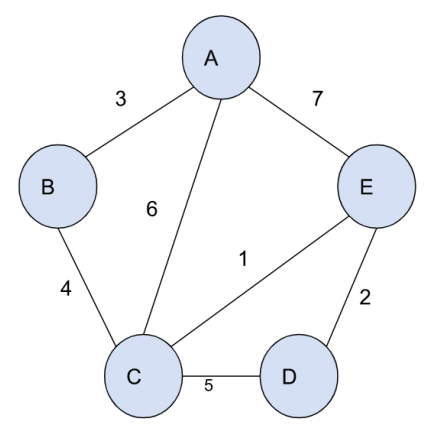
\includegraphics[width=0.35\linewidth]{HWs//HW11/figures/3.png}
\end{figure}
\vspace{-10pt}
\begin{itemize}
    \item[(a)] If we run Kruskal’s algorithm in the graph, what will be the sequence in which edges are added to the MST? \\
    \myAnswer{
    The sequence will be $\{(C, E), (D, E), (A, B), (B, C)\}$
    }
    \item[(b)] Demonstrate Prim’s algorithm in the graph with A as the source.
    \myAnswer{
    \begin{enumerate}
        \item At first, solution vertex set $S = \{A\}$. Now the accessible edge with minimum weight is $(A, B)$, so we add $B$ to $S$.
        \item $S = \{A, B\}$. Now the accessible edge with minimum weight is $(B, C)$, so we add $C$ to $S$.
        \item $S = \{A, B, C\}$. Now the accessible edge with minimum weight is $(C, E)$, so we add $E$ to $S$.
        \item $S = \{A, B, C, E\}$. Now the accessible edge with minimum weight is $(D, E)$, so we add $D$ to $S$.
        \item In the end, the final soulution set $S = \{ A, B, C, D, E\}$ \\
    \end{enumerate}
    }
\end{itemize}